\documentclass {article}
\usepackage {graphicx}
\usepackage [numbers]{natbib}

\begin {document}

\begin {figure}
\centering 
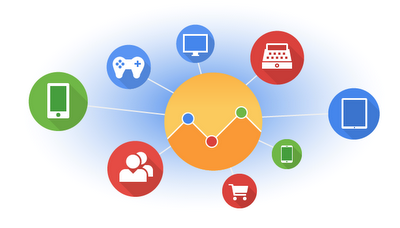
\includegraphics[scale=0.3]{googleanalytics.png}
\label {Photo1}
\end {figure}


\title {Google Analytics}
\author {Stephen Gift Mukoya Araka}
\maketitle 

\begin {abstract}
This is a short documentation about my reasearch about the Google Analytics product from Google.
\end {abstract}


\section {Introduction}
Google Analytics is a \cite{plaza2011google} freemium web analytics service offered by Google \cite{ghemawat2003google} that tracks and reports website traffic. Google launched the service in November 2005 after acquiring Urchin. Google Analytics is now the most widely used web analytics service on the Internet.

\subsection {The Technology}
Google Analytics is implemented with "page tags", in this case, called the Google Analytics Tracking Code, which is a snippet of JavaScript \cite{flanagan2006javascript} code that the website owner adds to every page of the website. The tracking code runs in the client browser when the client browses the page (if JavaScript is enabled in the browser) and collects visitor data and sends it to a Google data collection server as part of a request for a web beacon.

The tracking code loads a larger JavaScript file from the Google web server and then sets variables with the user's account number. The larger file (currently known as ga.js) is typically 18 KB. The file does not usually have to be loaded, however, due to browser caching. Assuming caching is enabled in the browser, it downloads ga.js only once at the start of the visit. Furthermore, as all websites that implement Google Analytics with the ga.js code use the same master file from Google, a browser that has previously visited any other website running Google Analytics will already have the file cached on their machine.


\subsection {Platform components}
Developers interact and influence processing through a rich user interface, client libraries, and APIs that are organized into 4 main components: collection, configuration, processing, and reporting.


\textbf{Collection}
collects user-interaction data.


\textbf{Configuration}
allows you to manage how the data is processed.


\textbf{Processing}
processes the user-interaction data, with the configuration data.


\textbf{Reporting}
provides access to all the processed data.


\begin {figure}
\centering 
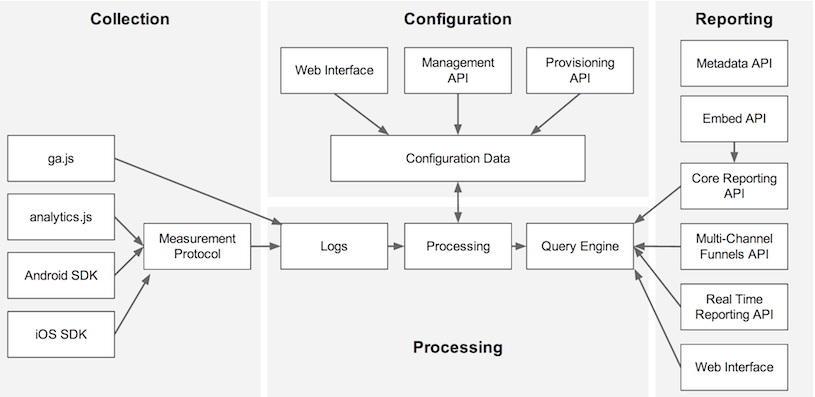
\includegraphics[scale=0.3]{example.png}
\caption {how it works.}
\label {Photo2}
\end {figure}

\section{User experiences}
When I \cite{clifton2012advanced} worked for a search engine marketing company, we would advise our clients to get this tool and they would exclaim, “I’ve never heard of such a thing!” They would say, “what is Google Analytics? How does it work?”

Information is from Wikipedia. \cite{wikipedia}

\bibliographystyle{IEEEtr}
\bibliography{References}

\end{document}